%=========PROBLEM 3============================================
\section*{Problem 3}

The AzTEC mm-wavelength camera completed a large survey of the COSMOS field in search for sub-millimeter galaxies. 
A typical source detection is between 4 and 10 sigma level. 

In this problem, the data composed of the signal to noise ratio is given. We need to produce an image of the data within 20 arc-minutes. In addition, we need to identify the source candidates with signal to noise ratio grater than 4.5.
The pixel size is $3 \times 3$ arc-seconds.

The steps followed to do the image are very similar to Problem 2:

\begin{enumerate}
    \item Import fit file and read header.
    
    Same as before
    
    \item Extract sky coordinates.
    
    As mentioned previously, the header contains metadata of the image including the coordinates in pixels of a reference pixel and its corresponding coordinates in the sky. All of these information, among others, is used to create a "projection" of the pixels into sky coordinates which is later use when plotting the data.
    
    \item Extract the data of the centered 20 arcminutes.
    
    Same as before.
    
    \item Create image of signal to noise ratio with a color bar.
    
    During initialization of the figure is necessary to include the command \lstinline[columns=fixed, style=Python]{projection=wcs}. This command will allow that the plot will show on world coordinates instead of pixel coordinates. It also allows that future x and y values can be given in both coordinate systems. 
    
    The command \lstinline[columns=fixed, style=Python]{imshow()} is used. Since the pixel is $3 \times 3$, it means is square so \lstinline[columns=fixed, style=Python]{aspect='equal'} is used so that the x and y axis have the same size. 
    
    \item Add circles to source candidates.
    
    To do this, is necessary to first determine the coordinates of such sources. The command \lstinline[columns=fixed, style=Python]{np.where(data>4.5)} returns the values of the pixels that satisfy the inequality. This x and y values are use in a scatter plot with the property facecolor='none'. Consequently, circles are plotted on source candidates. 
    
    Improvements needed: For sources that extend to more than one pixel, the center coordinate needs to determined so instead of having several circle squish together, it'll show a single circle around the source candidates. 
    
    \item Customize plot
    
\end{enumerate}

The image of the signal to noise ratio is shown on Figure \ref{fig:image}.

 \begin{figure}[h]
        \centering
        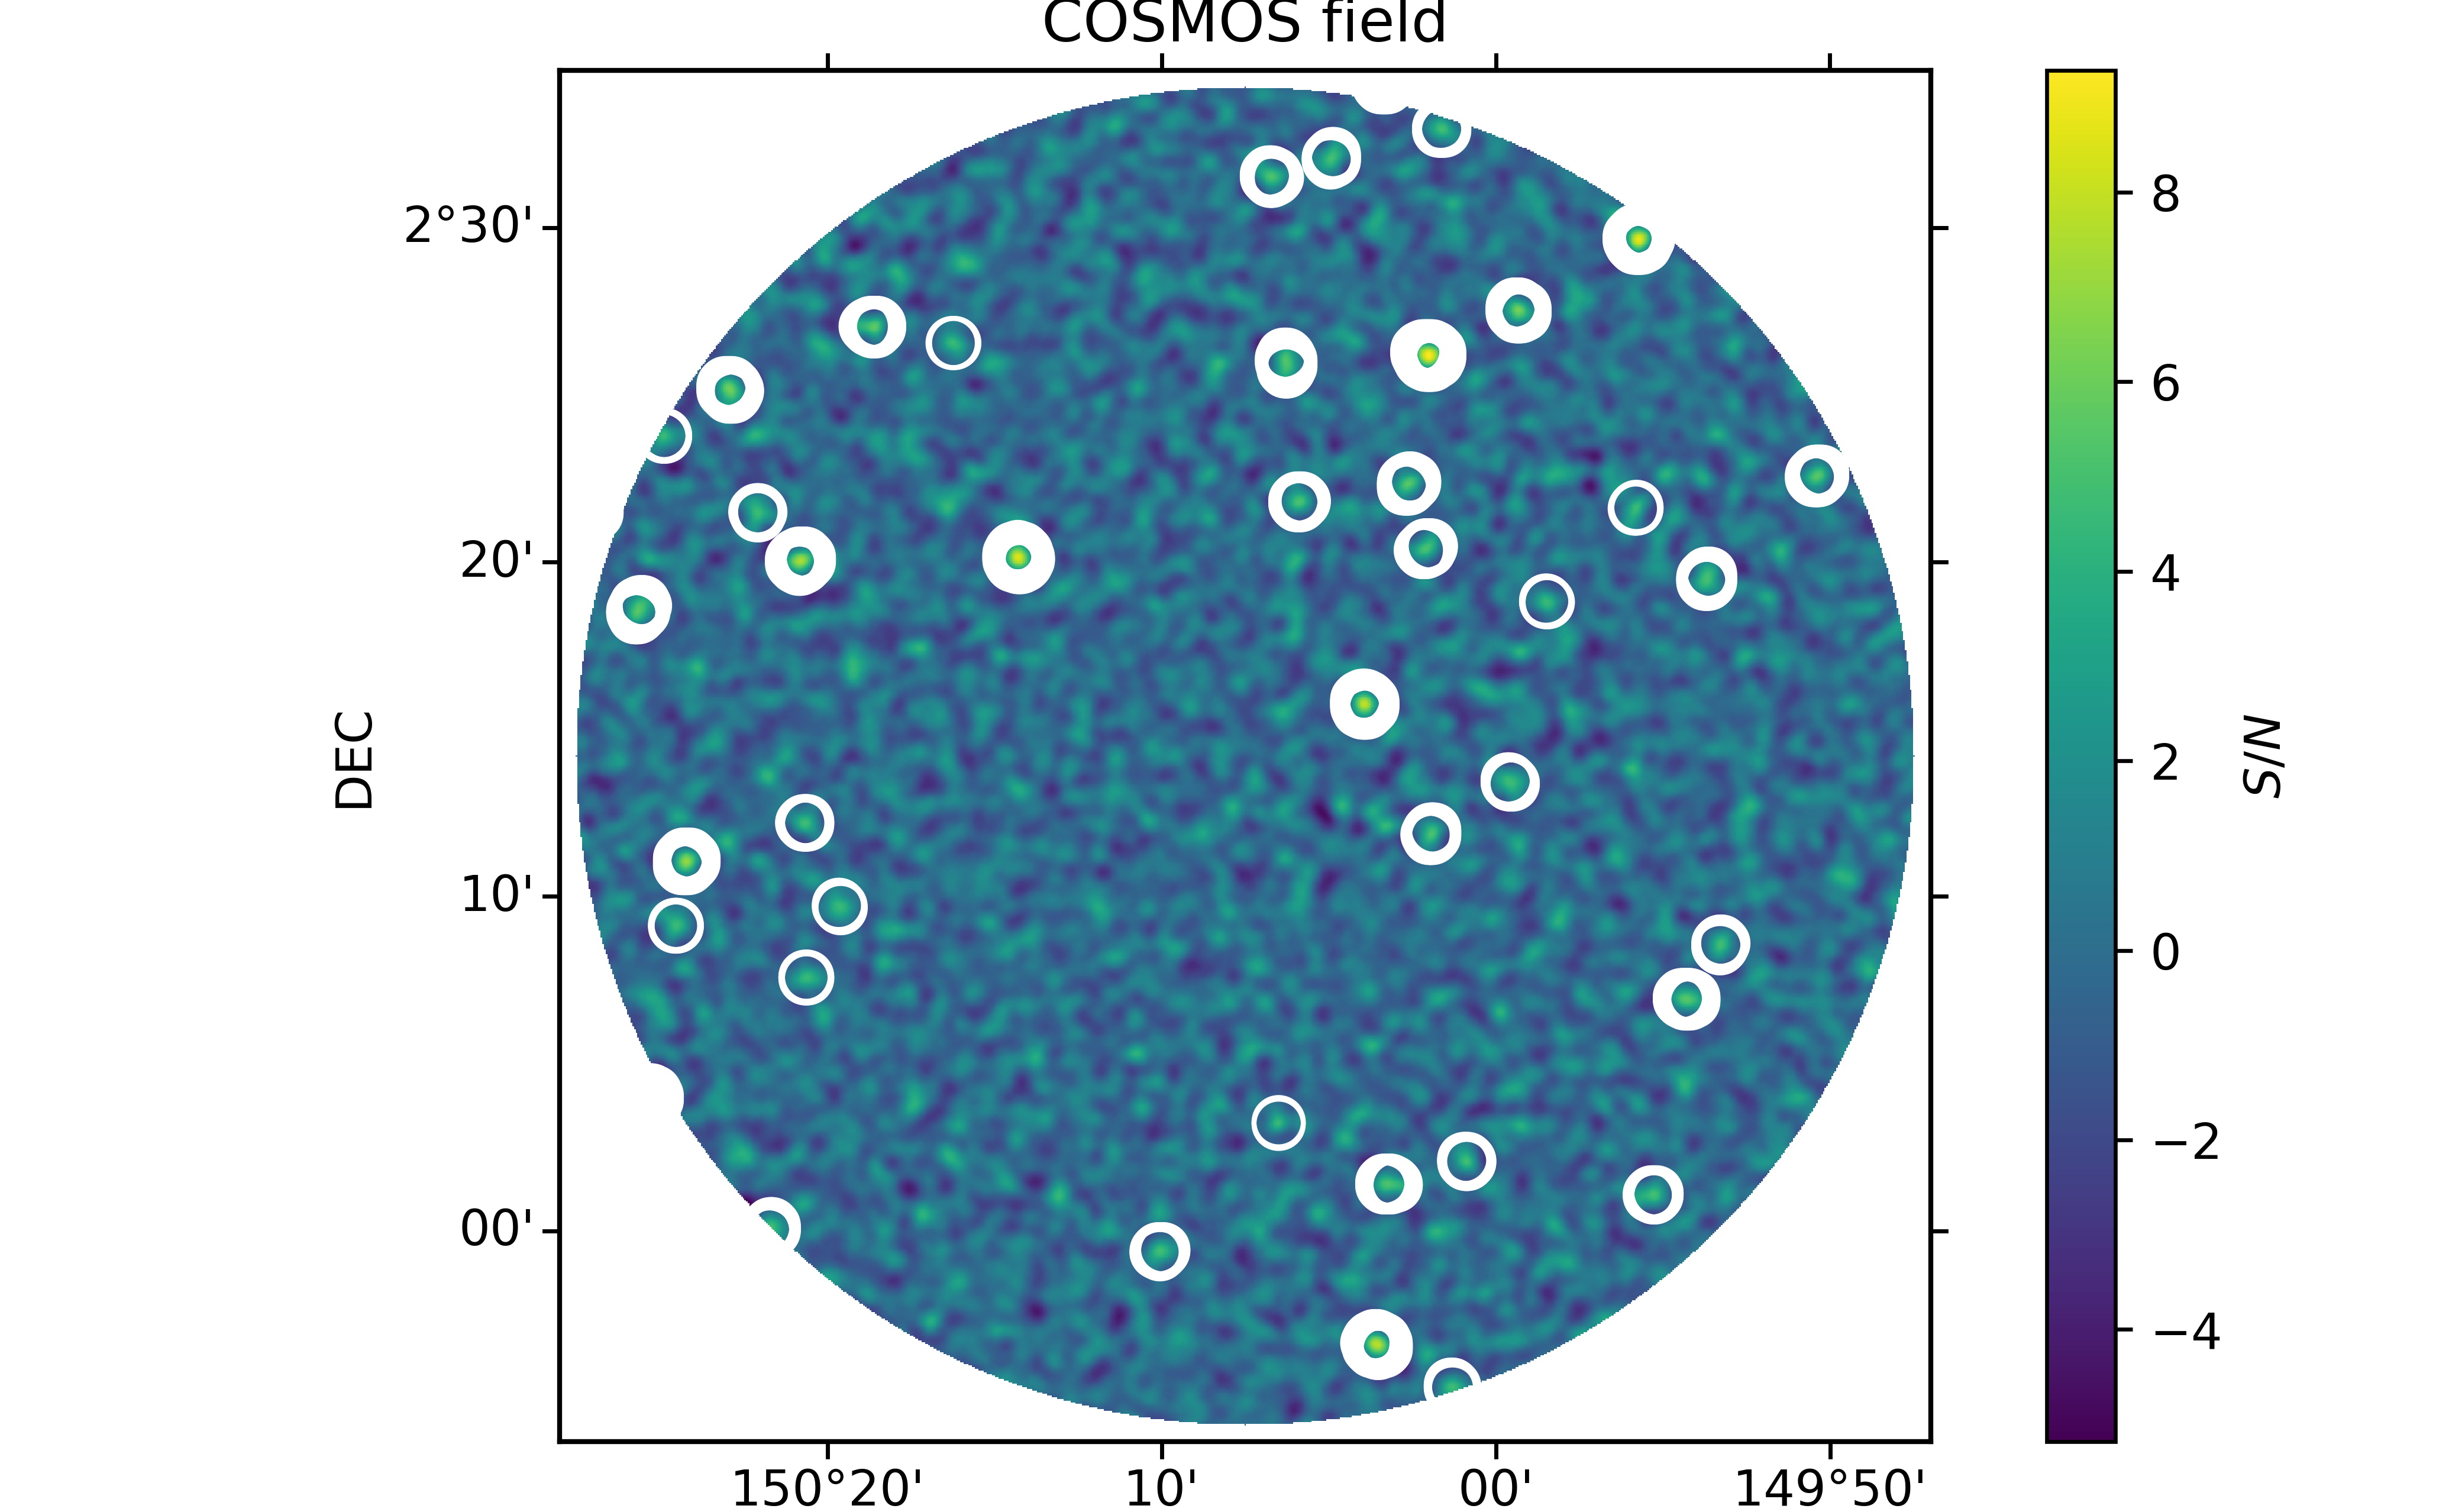
\includegraphics{figures/hw01prob1-3fig1.png}
        \caption{Signal to Noise Ratio of COSMOS field using AzTEC.}
        \label{fig:image}
    \end{figure}


%     